\part{Interaction Sol - Structures}

Un problème sol-structure apparaît lorsque l'équilibre dépend des raideurs relatives. On a donc un problème hyperstatique. Il existe plusieurs modèles pour le résoudre:

\begin{itemize}
    \item Règles de bonne pratique
    \item Approche avec hypothèse forte (structure souple ou rigide)
    \item Vérification des effets de la déformation libre sur la structure
    \item Méthodes numériques
    \item Méthode simplifiées au coefficient de raideur
\end{itemize}

\medskip

Nous on s'intéresse aux méthodes simplifiées (comme de par hasard !). Elles sont utiles en phase de conception car:

\begin{itemize}
    \item Plus fine que les méthodes de répartition arbitraire des contraintes de contact
    \item Elles mettent l'accent sur ce qui est essentiel (il y aura des coefficient de sécurité)
    \item Elles ne s'ennuient pas avec 15000 coefficient pour décrire la géométrie exacte
\end{itemize} 

\section{Détermination du coefficient de raideur et du module de réaction}

Le coefficient de raideur est le rapport contrainte/déplacement à l'interface, il est positif:

\begin{center}
\begin{tabular}{c|c}
    $ K = \frac{\Delta p}{\Delta s} = \frac{q}{w} \frac{[kPa]}{[mm]} $  
                & $\Delta p$: accroissement des contraintes \\
                & $\Delta s$: déplacement vers le sol 
\end{tabular}
\end{center}

Le module de réaction par rapport à la charge linéaire/déplacement:

    $$ E_k = \frac{p'}{\Delta s} = \frac{p}{y} \frac{[kN/m]}{[mm]} $$    

Il existe plusieurs méthodes pour définir ces coefficient que nous allons voir maintenant.

\subsection{Essai à la plaque}

Essai géotechnique donnant des infos sur la portance du sol.

\subsubsection{Description générale}

plaque circulaire de 200 cm² à 750 cm² suivant la granulométrie. On applique des charges par palier (essai statique) en fonction de la vitesse verticale (si $v \leq v_{min}$ on change). Une surcharge est appliquée pour assurer un contact uniforme. L'enfoncement est mesuré au moyen de capteurs fixés sur un support non solidaire du mouvement du sol. On mesure la charge grâce à un dynamomètre qu'on divise par l'air de la plaque pour obtenir une contrainte moyenne. On peut ainsi créer une courbe contrainte-tassement.

Il y a un exemple pages 4 et 5 du syllabus.

\subsubsection{Résultats de l'essai}

Dans la plupart des cas, la relation contrainte-tassement n'est pas linéaire. L'évolution est d'autant plus progressive que le matériau est bien compacté et proche d'une teneur en eau optimale. Il faut faire attention, le diamètre de la plaque fait varier le bulbe d'influence, il faut en tenir compte.

En pratique le module de réaction k est la pente de la sécante définie par un point de la courbe contraintes-déplacements.

Les praticiens calculent un nouveau coefficient: le coefficient de compressibilité à la plaque:
\begin{center}
\begin{tabular}{c|c}
$M_E [MPa] = D[m] \frac{\Delta p [kPa]}{\Delta s [mm]}$
                & D: diamètre de la plaque \\
                & $\Delta p$: accroissement de la pression \\
                & $\Delta s$: accroissement du tassement
\end{tabular}
\end{center}

Il est conseillé de calculer m, le rapport entre le coefficient de compressibilité du deuxième et du premier cycle. Si m < 2 et $M_E$ est faible, cela indique une mauvaise qualité du matériau.

\begin{center}
\begin{tabular}{c|c}
        $M_E [MN/m^2]$  &   Portance    \\
        >60             &   Très élevée \\
        <6              &   Très faible 
\end{tabular}
\end{center}

\subsubsection{Tassement d'une fondation suivant la théorie de l'élasticité}

Hypothèse: Le massif sous-jaçant est un milieu élastique isotrope homogène et N se réparti uniformément.

Selon Kérisel:
\begin{center}
\begin{tabular}{c|c}
$w = \frac{3.6 N}{E \zeta}$
                & w: tassement \\
                & N: charge appliquée \\
                & $\zeta$: périmètre de la surface de chargement \\
                & E: module de Young du massif
\end{tabular}
\end{center}

\begin{center}
\begin{tabular}{c|c}
$k = \frac{E \zeta}{3.6 S}$
                & k: coefficient de raideur \\
                & S: Surface 
\end{tabular}
\end{center}

On observe que si la taille de la surface augmente (effet d'échelle), le bulbe également et donc le tassement diminue. K diminue donc avec la taille de la plaque. La taille de la plaque à donc une réelle influence sur l'essai.

Un autre phénomène est l'augmentation du module de Young après un chargement. Quelle valeur de E adopter (drainé, non drainée, compression, cisaillement,...)? C'est a définir en fonction du cas de figure et des observations faites sur le terrain.

\subsubsection{Expériences}

Pour les sols sableux:

\begin{center}
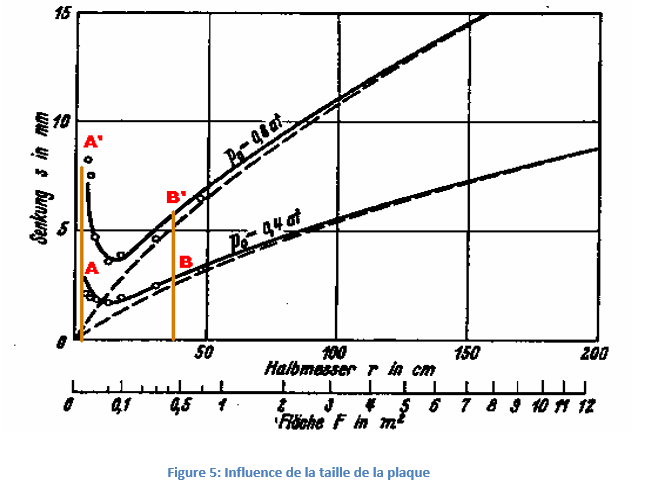
\includegraphics [scale=0.5]{pictures/5.PNG}
\end{center}

\begin{itemize}
    \item A: correspond à un essai CBR (California Bearing Ratio) poinçon de 500mm de diamètre. lois de déformation en plasticité qui gouvernent le tassement.
    \item B: plaque de 38cm de rayon, seules les zones en bordure de la plque sont en plasticité. On s'approche d'un comportement élastique homogène.
\end{itemize}

\medskip

On introduit une formule de correction qui fait ressortir une courbe asymptotique dessiné en traits tirés sur la figure précédente. Terzaghi et Peck on utilisé cette asymptote pour trouver une équation:

\begin{center}
\begin{tabular}{c|c}
$w = w_{30}(\frac{2B(')}{B(')+l'})^2$
        & $w_{30}$: tassement d'une plaque de référence \\
        & l':30.5 cm \\
        & B: largeur de la fondation (en pieds)
\end{tabular}
\end{center}

Il y a un manque de précision dans la prise de mesure (pas assez nombreuse). Il y a notamment un problème de mise à l'échelle du module de Young avec la profondeur.

\subsubsection{Formules empiriques}

Ces formules sont faites sur base d'essais et d'observations:

\paragraph{Argiles}

\begin{center}
\begin{tabular}{c|c}
$k=\frac{l'}{B(')}\frac{D(')+0.5'}{1.5D(')}k_l$
        & k: module de réaction \\
        & B: largeur (pieds) \\
        & D: la longueur (pieds) \\
        & $k_l$: module de réaction de référence 
\end{tabular}
\end{center}

\begin{center}
\begin{tabular}{c|c|c}
    Argile raide                & 1<lc          & $k_l'=96 MN/m^3$\\
    Argile moyennement raide    & 0.75<lc<1     & $k_l'=48 MN/m^3$\\
    Argile consistante          & 0.5<lc<0.75   & $k_l'=24 MN/m^3$
\end{tabular}
\end{center} 
    
\paragraph{Sables}

$$ k=(\frac{B(')+1}{2B})^2 k_l $$

\begin{center}
\begin{tabular}{c|c|c|c}
                                &                       & Au dessus     & En dessous    \\
    Sable lâche                 & $D_r < 0.33$          & $13 MN/m^3$   & $8 MN/m^3$    \\
    Sable moyennement compact   & $0.33 < D_r <0.66$    & $42 MN/m^3$   & $26 MN/m^3$   \\
    Sable dense                 & $0.66 < D_r$          & $160 MN/m^3$  & $96 MN/m^3$   
\end{tabular}
\end{center} 

\section{Poutre sur appui continu élastique}

\subsection{Hypothèses}

On considère une poutre de largeur B [m] et d'inertie I [$m^4$] soumise à des forces généralisées ponctuelles réparties. Transversalement, la pression est uniforme. Longitudinalement, la pression est proportionnelle à l'enfoncement et donc à la flèche ($p=kw$ hypothèse de Winkler). 

On considère le sol comme une succession de tranches transversales indépendantes agissant comme des ressorts verticaux.

\subsection{Équation différentielle}

On considère un élément de poutre de longueur élémentaire dx situé entre deux forces ponctuelles éventuelles et soumis uniquement à une charge répartie p. Elle subit donc les sollicitations suivantes:
\begin{itemize}
    \item p(x) une charge répartie par mètre de longueur [kN/m]
    \item $\sigma(x)$ la pression de contact avec le sol $[kN/m^2]$
    \item M et M+dM les moments aux extrémités
    \item N les efforts normaux constant (hypothèse) dus aux charges ponctuelles axiales, on néglige le cisaillement le long du sol.
    \item T et T+dT les efforts tranchants aux extrémités.
\end{itemize}

\begin{center}
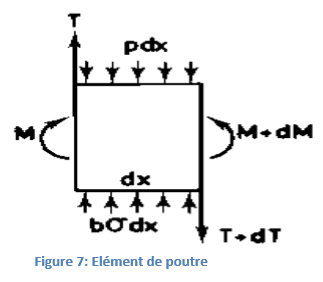
\includegraphics [scale=0.5]{pictures/7.PNG}
\end{center}

\underline{Équilibre de rotation:} $M(x,t)-M(x+\Delta x,t)+T(x,t)\Delta x =0$

\underline{$\sum F_y = 0$:} $T(x+\Delta x)-T(x) + b \sigma \delta x - p \Delta x =0$

On en tire que: 

\begin{center}
 $\frac{\delta T}{\delta x} = b \sigma-p $   \smallskip    et      $ T=\frac{\delta M}{\delta x} $ 
 \end{center}

Ce qui donne:

$$ \frac{\delta ^2 M}{\delta x^2} = b \sigma-p $$

Grâce à l'hypothèse de conservation de la planéité des sections transversales et que la poutre est supposé élastique ( + E connu), on peut dire que: 

$$ \frac{d ^2 w}{d x^2} = -\frac{M}{E I} $$

On injecte cette équation dans celle obtenue précédemment et on développe $\sigma$, on obtient ainsi l'équation différentielle du tassement:

$$ E I \frac{\delta ^4w}{\delta x^4}+kbw = p$$ 

\subsection{Solution générale}

C'est une somme de quatre fonctions de base:

$$ w(x) = c_1 f_1 + c_2 f_2 + c_3 f_3 + c_4 f_4 $$

il suffit de trouver la solution générale de l'équation rendue homogène et de trouver l'intégrale particulière, solution de l'équation complète qu'on ajoute à la solution générale de l'équation homogène (math 3). On remarque que grâce à l'hypothèse que la poutre sur un sol élastique permet de négliger le terme dû à l'excentricité des efforts normaux.

Raisonnement mathématique p 14, 15 et 16 du syllabus.

Solution:   avec $\lambda : (\frac{kb}{4 EI})^\frac{1}{4}$ 

\begin{itemize}
    \item (dérivé) pente ou rotation de la poutre: $\frac{1}{\lambda}\frac{dw}{dx} = l_e tan(\theta) : l_e \theta $
    \item (dérivé seconde) Moment M: $\frac{1}{2\lambda^2}(-EI\frac{d^2w}{dw^2} = M l_e^2$
    \item (dérivé troisième) Effort tranchant T: $\frac{1}{2\lambda^3}(-EI\frac{d^3w}{dx^3} = Tl^3_e$
    \item (hypothèse de Winkler) $\sigma = Kbw$
\end{itemize}
Attention il faut rajouter les constantes d'intégrations.

\subsection{Détermination des constantes - Méthode de Hetenyi}

On considère cette fois une poutre de longueur finie l dont l'extrémité coïncide avec l'origine du système d'axes (x,w). Elle reste chargée par les couples M, les charges ponctuelle P et une charge répartie p.

La démonstration se trouve p 17 et 18.

De toutes façons cette méthode a perdue son utilité pratique. On utilise des méthodes numérique pour résoudre ce genre de chose. Mais apparemment c'est vraiment une belle résolution d'équation.

\section{Charge excentrée et radiers}

\subsection{Charge Excentrée}

Une charge excentrée est équivalente à une charge centrée et un moment de force calculé en flexion composé. Il faut éviter l'apparition de contrainte de traction en s'assurant que la résultante Q reste dans le noyau.

Il arrive souvent que par suite de l'excentricité, l'équilibre limite soit atteint au bord extrême de la semelle.

\begin{center}
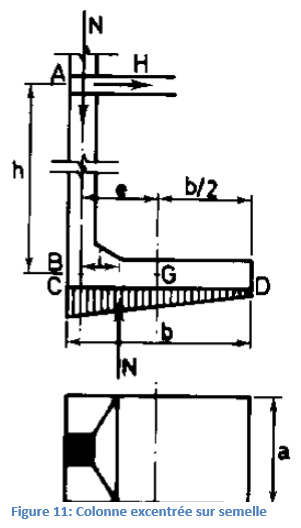
\includegraphics [scale=0.5]{pictures/11.PNG}
\end{center}

$\theta_b$: rotation de la base de la colonne lié rigidement à la semelle.

$$ \theta_b= \frac{M_B h}{3EI} = \frac{Q e h}{3EI}$$

$\theta_s$: rotation de la semelle supposée rigide.

$$ \theta_s=\frac{12Q(l-e)}{kLB^3} $$

En égalant ces deux équations, on obtient l'excentricité e:

$$ e = \frac{l}{1+\frac{kLhB^3}{36EI}} $$

On peut ainsi trouver les force $q_c$, $q_d$ et H. Si l'une de ces forces est en traction, on a un problème! il faudra alors soit augmenter le poids de la semelle, soit redistribuer la descente de charge ailleurs.

\subsection{Radier Général}

\begin{center}
\begin{tabular}{c|c}
$q=\frac{Q}{BL}(1\pm \frac{6c}{B} \pm \frac{6c'}{L}$
        & Q: charge décentrée \\
        & B: largeur \\
        & L: longueur \\
        & (c,c') coordonnée de la charge 
\end{tabular}
\end{center}

\subsection{Semelle sur pieux}

\begin{center}
\begin{tabular}{c|c}
$Q_i = Q(\frac{k_i}{\sum k_i}+e\frac{k_i r_i}{\sum k_i r_i^2}$
        & $Q_i$ l'effort du pieu i \\
        & $\sum k_i$: coefficient de réaction total \\
        & $r_i$: la distance vis-à-vis de l'axe neutre
\end{tabular}
\end{center}

\section{Pieux soumis à des efforts horizontaux}

\subsection{Pieux actifs et passifs}

\begin{itemize}
    \item Pieux actifs: pieux sollicité en tête et qui doit trouver sa réaction latéral dans le sol. Les efforts transmit sont des forces horizontales et des couples (du à la structure). Il en résulte un déplacement horizontal.
    \item Pieux passifs: Les pieux sont soumis à des efforts latéraux sous l'effet de déplacement du sol avoisinant. C'est le correspondant latéral du frottement négatif
\end{itemize}

\subsection{Conceptions des groupes de pieux soumis aux efforts latéraux}

incliner les pieux pour les faire travailler axialement. Ils ont une plus grande raideur axiale que transversale (à l'instar d'une colonne encastré à sa base). Il faut donc réfléchir à l'inclinaison des colonnes. Lorsque les efforts horizontaux sont limités (10\%), il reste possible de faire travailler les pieux en flexion.

\subsection{Pieux actifs}

Nécessite de l'itération parce que la réponse du sol n'est pas linéaire du déplacement de la structure.

La solution cherchée comprend:
\begin{itemize}
    \item y: le déplacement horizontal
    \item $\theta$: la pente
    \item M: le moment fléchissant
    \item T: l'effort tranchant
    \item P: la réaction horizontale
    \item dz: unité de hauteur.
\end{itemize}

\subsection{Réaction élastique linéaire}

On fait l'analogie avec le cas de la poutre continue appuyée sur ressort élastique vue précédemment. On reprend l'équation différentielle résultant de l'hypothèse de Winkler. Elle est applicable aux pieux unique ou groupe de pieux mais nécessite la connaissance du module de réaction latérale du sol vis-à-vis du pieu [MPa].

Dans le cas ou h>3$l_e$, le pieu est flexible et les déformations sont déterminées en résolvant l'équation différentielle homogène (il est alors nécessaire de vérifier que nulle part la contrainte dans le sol ne dépasse la limite élastique et que le moment fléchissant ne dépasse pas la limite imposé par la résistance du pieu).

Dans les exemples suivant, on a remplacé k par $\lambda$.

\paragraph{Pieu semi-infini non encastré soumis à un couple $M_0$}

$$M(z) = T_0 l_e e^{-\lambda z} sin(\lambda z)$$
$$M_max=T_0l_e exp(-\frac{\pi}{4})\frac{\sqrt{2}}{2} = 0.32 T_0 l_e $$ 

$$T(z) = -\frac{2M_0}{l_e} exp(-kz) sin(\lambda z)$$

\paragraph{Pieu semi-infini encastré soumis à une force horizontale $T_0$}

$$M(z)=-\frac{T_0 l_e}{2} exp(-kz) (cos \lambda z - sin \lambda z) $$
$$T(z) = T_0 exp(-kz) cos \lambda z$$

Moment maximal à l'encastrement: $M_max=0.5 T_0 l_e$ 

il change de signe à $\frac{\pi}{4} l_e$. Si un pieu dépasse trois fois la longueur élastique, on peu négliger les contraintes de déformations.

\paragraph{Valeurs en tête du pieu}

\begin{center}
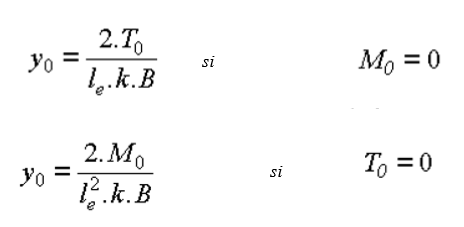
\includegraphics [scale=0.7]{pictures/abc.PNG}
\end{center}

\subsection{Courbes de réaction (P-y)}

La réponse du sol est non linéaire, on ne peu donc pas se limiter à la pente de la droite P/y. Le sol étant hétérogène et la pression dépendant de la profondeur on doit faire une courbe précise. On conserve le principe 'indépendance des réactions individuelles le long du pieu (on exclu l'influence des couches voisines). Ce problème revient à déterminer un module sécant $E_s$ correspondant à chaque valeur du déplacement horizontal y. Nous allons utiliser une méthode basées sur des essais sur modèles de pieux en laboratoire (Matlock, Reese, ...).

On va s'aider d'un déplacement de référence $y_50$ correspondant à la mobilisation de la moitié de la résistance ultime (FS=2).

\subsubsection{Méthode de Matlock pour des argiles molles}

B = 2R (diamètre du pieux), $c_u$ = cohésion et $\gamma$ = poids volumique.

\paragraph{Chargement simple}

honnêtement j'ai rien compris 

\paragraph{Chargement cyclique}

Matlock est trop optimiste, utiliser la méthode pressiométrique de Menard.

\subsubsection{Méthode de Reese et Welch pour les argiles raides}

\paragraph{Chargement simple}

fort semblable à Matlock mais cette fois, l'équation s'écrit:

$$ \frac{p}{p_u} = 0.5 (\frac{y}{y_50})^\frac{1}{4} $$

\paragraph{Chargement cyclique}

On fait appel à une fonction logarithmique du nombre N.

$$y_{cyclic} = y_{static} + y_{50} C log N $$

avec $y_{50}$ le déplacement à 50\% de la résistance ultime et $C=9.6(p/p_u)^4$ une constante.

\subsubsection{Méthode de O'Neil et Murchinson pour les sables}

On identifie une résistance latérale ultime sous la profondeur critique restant définie par unité de longueur du pieu. Un autre pour les zones proche de la surface. La profondeur critique s'obtient en égalent les deux expressions obtenues.

Cette méthode fait l'hypothèse dans un cas pulvérulent que la raideur initiale augmente linéairement avec la profondeur suivant la densité relative.

\paragraph{Validité des méthodes précédentes}

Matlock suggère une nappe phréatique affleurante alors que Reese et Welch on une nappe plus profonde, pas applicables aux structures offshore. 

\subsection{Pieux passifs}

\subsubsection{Méthode basé sur le module de réaction}

On résout par itération l'équation de Wikler. Fonctionne bien si on met des valeurs mesurée a posteriori. Si l'on place des solution calculée, il y a un écart important avec la réalité.

\subsubsection{Méthode semi-empirique}

Plusieurs auteurs ont constaté que lorsque le coefficient F de sécurité vis-à-vis de la rupture s'ensemble reste supérieur à 1.4 les déplacement horizontaux à la surface semblent obéir à une loi élastique dépendant fortement du rapport H/B (épaisseur H et largeur B). Lorsque le facteur est inférieur, les déplacements croissent considérablement.
